%Queremos hacer en el formato IEEE
%Entonces requeriremos de otra entrada diferente a la usual...
% \documentclass[11pt,a4paper]{article}

%Nos hemos guiado de una plantilla ejemplo.

\documentclass[journal]{IEEEtran}
\hyphenation{op-tical net-work semi-conduc-tor}%PARA arreglar el abstract y los romanos
%\documentclass[letterpaper, 10 pt, conference]{ieeeconf}


\IEEEoverridecommandlockouts  

%\overrideIEEEmargins %Para equilibrar las columnas

%\usepackage[utf8]{inputenc}
%\usepackage{amsmath}
%\usepackage{amsfonts}
%\usepackage{amssymb}
%\usepackage{multicol}
\usepackage{graphicx}
%\usepackage{multicol}
\usepackage{endnotes}
\title{\LARGE \bf
		Verificación de la existencia de un ciclo Hamiltoniano en un grafo aleatorio}




%%%%%%%%%%%%%%%%%%%%%%%%%%%%%%%%%%%%%%%%%%%%%%%%%%%%%%%%%%%%%%%%%%%%

\begin{document}

\maketitle
{Maquera Briguitte\footnote{E.P. de Matemática-Facultad de Ciencias, 	Universidad Nacional de Ingeniería, briguittemaquera@gmail.com, código 20162254B}, Farut Jaafar\footnote{E.P de Facultad de Ciencias, 	Universidad Nacional de Ingeniería, jaafarsahua@hotmail.com, código 	20161395A} y Rivera Franklin\footnote{E.P de Ciencias de la Computación, Facultad de Ciencias, Universidad Nacional de Ingeniería, friverag@uni.pe, código 20161331C}}
\vspace{10mm}
\thispagestyle{empty}

\pagestyle{empty}


%%%%%%%%%%%%%%%%%%%%%%%%%%%%%%%%%%%%%%%%%%%%%%%%%%%
\begin{abstract}
	
	The project deals with the implementation of an algorithm that helps us to verify if a random graph is Hamiltonian with the help of the igraph package, libraries and functions that they offer in R language.
\end{abstract}

\begin{abstract}
	
	El proyecto trata sobre la implementación de un algoritmo que nos ayude a comprobar si un grafo aleatorio es Hamiltoniano  con la ayuda del paquete \textit{igraph}, librerias y funciones que ofrecen en lenguaje R. 

\end{abstract}

%%%%%%%%%%%%%%%%%%%%%%%%%%%%%%%%%%%%%%%%%%%%%%%%%%%%%	
	
\section{\large\bf INTRODUCCI{\'O}N}
 
 {\bf Objetivos:}\\
 \begin{enumerate}
 	\item El objetivo de nuestro proyecto es encontrar si existe o no un {\bf Ciclo Hamiltoniano} en un grafo aleatorio dado sus números de aristas y vertices con ayuda de los paquetes que R ofrece.
 	
 \end{enumerate}
\vspace{0.2mm}
{\bf Definiciones previas}\\
\vspace{0.2mm}

• \textbf{Grafo}: Es un diagrama que representa mediante vertices y aristas las relaciones entre pares de elementos y que se usa para resolver problemas l{\'o}gicos, topol{\'o}gicos y de c{\'a}lculo combinatorio.\\

\vspace{0.2mm}
• \textbf{Grafo hamiltoniano}: Es aquel grafo que tiene un ciclo hamiltoniano el cual recorre una sola vez cada vertice y el vertice final sea adyacente al primero, de esa forma contiene un camino hamiltoniano o circuito hamiltoniano.\\


•\textbf{¿{C{\'o}mo identificar un grafo hamiltoniano}?}\\
Contrario al caso de los grafos eulerianos, para el caso de los grafos hamiltonianos no se conoce ninguna condici{\'o}n necesaria y suficiente que los caracterice. Esto es lamentable porque en muchas aplicaciones es fundamental poder determinar si un grafo es hamiltoniano.\\
\vspace{1cm}

•\textbf{¿{Qu{\'e} es el Lenguaje de programaci{\'o}n R}?}\\

Es un tipo de lenguaje de programaci{\'o}n el cual es una implementaci{\'o}n del lenguaje de programaci{\'o}n S, creado en Auckland(New Zealand)\\

Caracter{\'i}sticas:\\
\textbf{*} R es un lenguaje pensado para la programaci{\'o}n estad{\'i}stica y la creaci{\'o}n de gr{\'a}ficos\\
\textbf{*} Posee mucho paquetes y librerias\\
\textbf{*} Es multi-paradigm{\'a}tico y Open Source ya que nos permite una facilidad en el uso de la escritura o implementaci{\'o}n del c{\'o}digo\\
\textit{\textbf{Nota:}}RStudio es un entorno de desarrollo integrado (IDE) para el lenguaje de programación R, dedicado a la computación estadística y gráficos.\\


%%%%%%%%%%%%%%%%%%%%%%%%%%%%%%%%%%%%%%%%%%%%%%%%%%%%%%%%%%%%%%%%%%%%%%%%%%%%%
 
\section{\large\bf ESTADO DEL ARTE}

\begin{enumerate}
\item El problema respecto a los grafos, espec{\'i}ficamente los ciclos hamiltonianos, vienen siendo una adversidad hist{\'o}rica.\\
En \textbf{1736} Leonhard Euler en uno de sus viajes en Koñigsberg en la costa del Mar B{\'a}ltico, en la Prusia oriental (Rusia) hab{\'i}an siete puentes distribuidos donde plane{\'o} un paseo de manera que saliendo de casa cruce los siete puentes una sola vez cada uno antes de regresar a casa haciendo referencia a los caminos hamiltonianos.\\
En \textbf{1805} Roman Hamilton se propuso a viajar a 20 ciudades del mundo, representadas como los v{\'e}rtices de un dodecaedro regular, siguiendo las aristas del dodecaedro.\\
En \textbf{1824} Kirchoff se sirvi{\'o} de la Teor{\'i}a de Grafos para enunciar las leyes que permiten el c{\'a}lculo de voltajes y circuitos el{\'e}ctricos.

\item \textbf{Network Analysis and Visualization with R and igraph}\\
 This page gave us information about the various functions that we can use in Rstudio and also about the igraph package which will help us in the graph drawings in Rstudio\\

\end{enumerate}

%%%%%%%%%%%%%%%%%%%%%%%%%%%%%%%%%%%%%%%%%%%%%%%%%%%%%%%%%%%%%%%%%%%%%%%%%%%%%%%%%%%

\section{\large\bf DISE\~{N}O DEL EXPERIMENTO}
\subsection{¿Es G hamiltoniano?}
\begin{itemize}
	\item No existe ningún método general v{\'a}lido aplicable a todos los grafos para determinar si es o no hamiltoniano.
	\item	El m{\'e}todo que trataremos a continuaci{\'o}n es válido, en t{\'e}rminos generales, si el grafo tiene v{\'e}rtices de grado dos y no tiene un gran n{\'u}mero de aristas (aunque la aplicabilidad o no del m{\'e}todo depende siempre del grafo en concreto).
\end{itemize}

\subsection{¿Qué m{\'e}todo utilizaremos?}
\begin{itemize}
	\item El m{\'e}todo será constructivista, buscando no s{\'o}lo la existencia sino el ciclo hamiltoniano, caso de que exista.
\end{itemize}

\subsection{¿En qu{\'e} se apoya?}
\begin{itemize}
	\item El m{\'e}todo se apoya en el hecho de que existe un ciclo hamiltoniano, éste debe contener exactamente dos de las aristas de cada uno de los v{\'e}rtices (por definición de ciclo).
\end{itemize}

\subsection{Estrategia}
\begin{itemize}
	\item	Dado un grafo no dirigido G, con $|v|>2$, suponemos que tiene ciclo hamiltoniano e intentaremos construirlo a partir de cuatro reglas.
	\item	Si las reglas 1 o 4 no se cumplen, el grafo no ser{\'a} hamiltoniano.
	\item En caso contrario habremos obtenido, tras un n{\'u}mero determinado de pasos, un ciclo hamiltoniano en G.
\end{itemize}

\subsection{Reglas}
	Suponemos que existe un ciclo hamiltoniano C en G.
\begin{enumerate}
	\item[Regla 1:]  Si existe ciclo hamiltoniano en G entonces todos los v{\'e}rtices tienen grado mayor o igual que dos.
	\item[Regla 2:] Sea v un v{\'e}rtice de grado 2. Entonces las dos aristas incidentes en v deben pertenecer al ciclo C.
	\item[Regla 3:] Si v es un vértice de grado mayor que 2, y ya hemos incorporado al ciclo C que estamos reconstruyendo dos de sus aristas, el resto de aristas incidentes en v deben ser desechadas.
	\item[Regla 4:] Si el grafo es realmente hamiltoniano, con la construcci{\'o}n obligada que estamos realizando no podemos encontrar un ciclo que contenga un número de vértices menor que $|v|$.
\end{enumerate}

\section{\large\bf IMPLEMENTACI{\'O}N EN R}

\subsection{Funciones y t{\'e}cnicas a usar}

\begin{enumerate}
	\item{\bf Plot:}\\ La funci{\'o}n plot es una función gen{\'e}rica para la representaci{\'o}n gr{\'a}fica de objetos en R. Los gr{\'a}ficos m{\'a}s sencillos que permite generar esta funci{\'o}n son nubes de puntos (x, y).
	
	\item{\bf Grafos con igraph:}\\ El paquete para Igraph, necesita que se le presente los datos de la matriz de adyacencia por parejas. Es decir, una matriz de doble entrada convencional (tambi{\'e}n llamada sociomatriz, tabla de confundido o tabla de concordancia) ha de pasarse al formato de igraph.
	
	\item{\bf Archivos CSV:}\\ Archivo de texto que contiene una serie de valores separados por comas. Los valores pueden ser cualquier cosa, desde n{\'u}meros de un presupuesto de una hoja de c{\'a}lculo, hasta nombres y descripciones de una lista de clientes de un negocio.
	
\end{enumerate}
\section{\Large{\bf EXPERIMENTOS Y RESULTADOS}}
\begin{figure}
	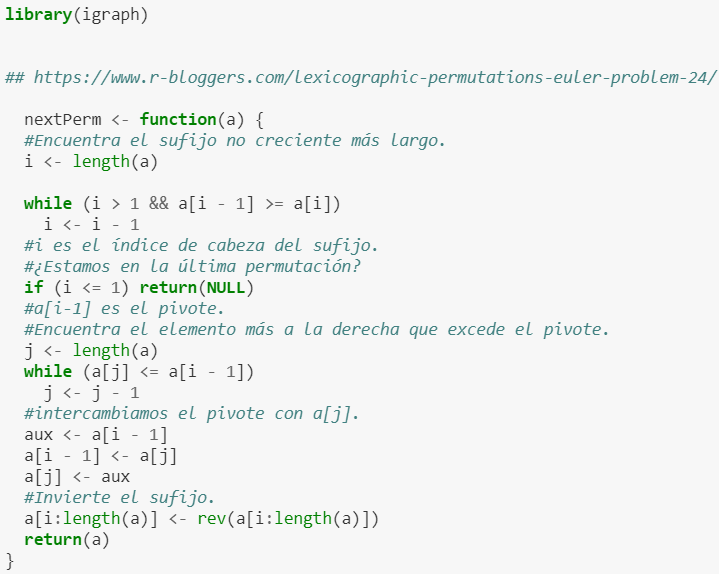
\includegraphics[scale=0.5]{parte_1.PNG}
	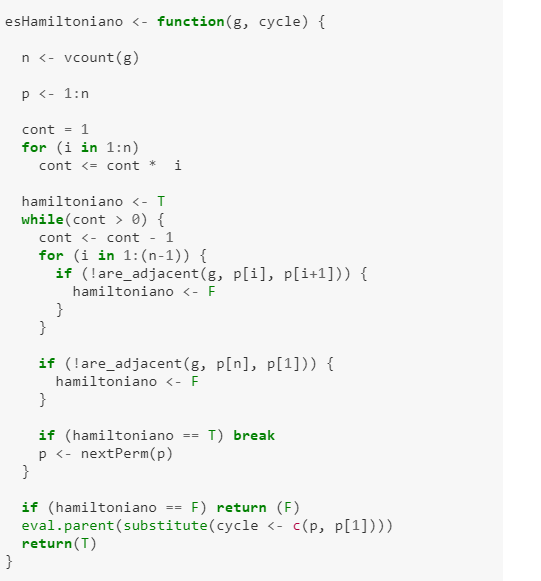
\includegraphics[scale=0.5]{parte_2.PNG}
	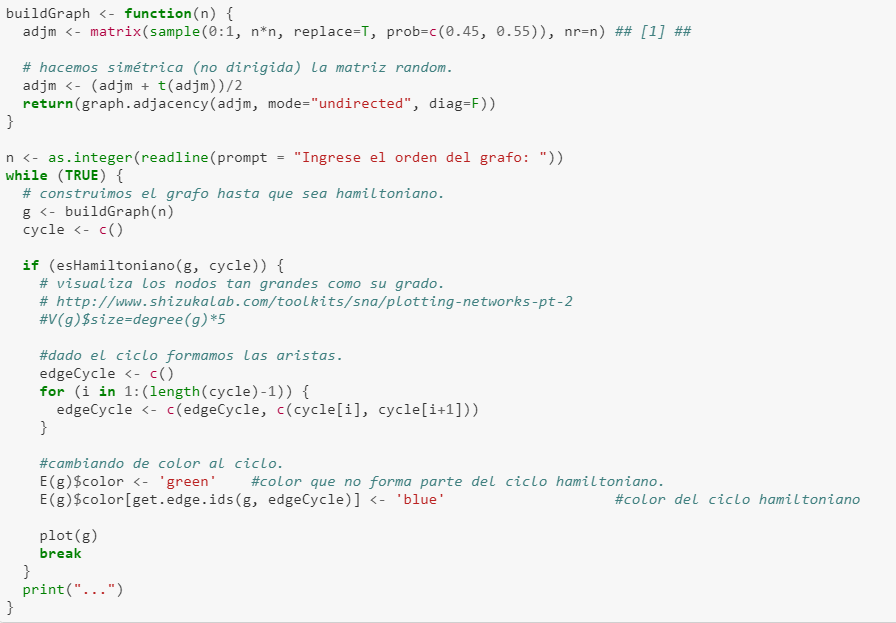
\includegraphics[scale=0.5]{parte_3.PNG}
\end{figure}
\newpage



\begin{figure}
	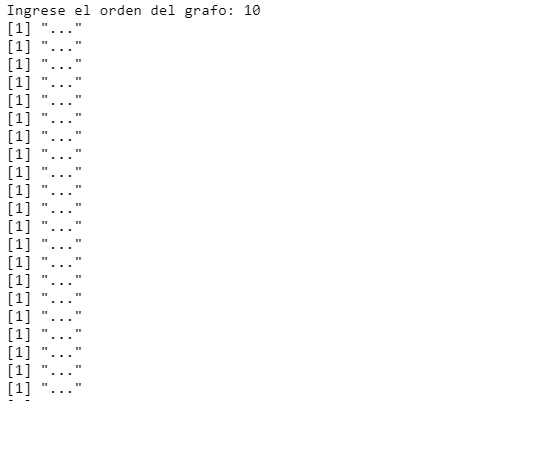
\includegraphics[scale=0.5]{parte_4.PNG}
	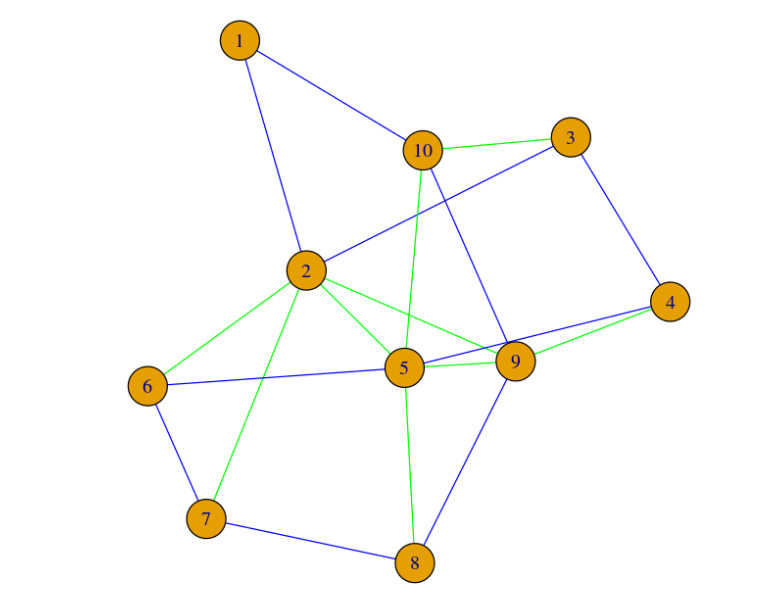
\includegraphics[scale=0.5]{parte_5.PNG}
\end{figure}
\section{\Large{\bf DISCUSIONES}}
\begin{enumerate}
	\item Al ejecutar el c{\'o}digo nos solicitar{\'a} el n{\'u}mero v{\'e}rtices n.
	\item luego se procede a construir el grafo aleatorio:
	Usando la funci{\'o}n \textbf{sample()} generamos $n*n$ n{\'u}meros aleatorios entre 0 y 1 , luego con la funci{\'o}n \textbf{matrix()} creamos una matriz(\textbf{adjm}) a partir del conjunto de valores obtenidos el cual ser{\'a} nuestra matriz de adyacencia. luego hacemos sim{\'e}trica la matriz usando la propiedad \textbf{(adjm + t(adjm)/2}.
	\item Luego pasamos a verificar si el grafo obtenido es hamiltoniano:\\
	Entraremos a un bucle en el cu{\'a}l su peor caso será n!, donde en el primer \textbf{for} usando la funci{\'o}n \textbf{$are\_adjacent()$} con el cual verificaremos si los v{\'e}rtices de las posiciones 1 hasta n-1 son adyacentes es decir si est{\'a}n conectados por un camino y por {\'u}ltimo verificamos si los v{\'e}rtices de la posici{\'o}n 1 y n son adyacentes. En caso no se cumpla lo anterior nos apoyamos de la funci{\'o}n \textbf{nextPerm()}  para permutar los v{\'e}rtices y seguir con el paso anterior hasta conseguir el grafo deseado.
	
	\item ¿C{\'o}mo se puede mejorar sus resultados?\\
	La complejidad del {\'o}digo es n! por lo cual es muy ineficiente y una manera de mejorarlo es optimizandolo e incluso se podría bajar hasta O(nlogn).
\end{enumerate}
\section{\Large {\bf CONCLUSIONES}} 
Se pud{\'o} implementar un código en R y utilizando el paquete igraph(principalmente la función plot) que R nos ofrece se pudo visualizar dicho grafo aleatorio y verificar que era hamiltoniano.
\begin{thebibliography}{X}
	\bibitem{clave-1} \textbf{Libro}: \textit{Invitaci{\'o}n a Matem{\'a}tica Discreta} \\  \emph{Autores}: "Jiri Matousek y Jaroslav Nesetril", (2008) \textit {Universidad de Charles-Praga}, \textbf{p{\'a}ginas}: 105-142
	\bibitem{clave-2} \textbf{Pagina Web-Video}: https://www.youtube.com/watch?v=LcL-tO2TMlY
	\bibitem{clave-3} \textbf{Pagina Web-Art{\'i}culo PDF}: https://www.ugr.es/~batanero/pages/ARTICULOS/libroR.pdf
	\bibitem{clave-4}   \textbf{Libro}: \textit{El arte de programar en R (Un lenguaje para la estad{\'i}stica)} \\  \emph{Autores}: "Julio Sergio Santana y Efra{\'i}n Mateos Farf{\'a}n ", (2014) \textit{Instituto Mexicano de Tecnolog{\'i}a del agua}
	\bibitem{clave-5} \textbf{Referencias del c{\'o}digo:} \\
		\begin{enumerate}
		\item https://www.r-bloggers.com/lexicographic-permutations-euler-problem-24/ \\
		\item http://igraph.org/r/doc/ \\
		\item https://stat.ethz.ch/R-manual/R-devel/library/base/html/bitwise.html \\
		\item https://stackoverflow.com/questions/4678333/nn-1-what-does-this-expression-do \\
		\item https://www.r-graph-gallery.com/248-igraph-plotting-parameters/ \\
		\item http://www.shizukalab.com/toolkits/sna/plotting-networks-pt-2 \\
	\end{enumerate} 
\end{thebibliography}

\end{document}

